\documentclass{standalone}
\usepackage{tikz}
\begin{document}
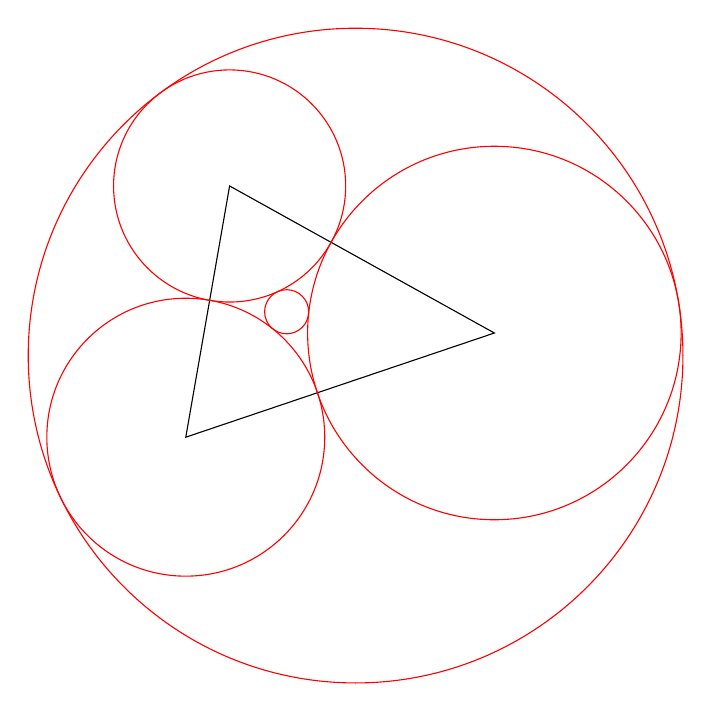
\begin{tikzpicture}[x=1pt,y=1pt]
\draw (202.51,-132.05) -- (91.00,-169.70) -- (106.84,-78.92) -- cycle;
\draw[red] (91.00,-169.70) circle (50.21);
\draw[red] (202.51,-132.05) circle (67.48);
\draw[red] (106.84,-78.92) circle (41.94);
\draw[red] (127.45,-124.37) circle (7.96);
\draw[red] (152.36,-140.21) circle (118.29);
\end{tikzpicture}
\end{document}
